\subsection{Beta-Strahlung}

Verwendet wird ein $^{90}\text{Sr}$ Strahler, der $\beta$-Teilchen mit einer Energie
von ungefähr $\SI{0.546}{\mega\electronvolt}$ emittiert. Der Strahler ist ein
reiner $\beta$-Strahler und ein $\beta$-Zerfall erfolgt nach dem Schema

\begin{align*}
    n \to p + e^{-} + \bar{\nu} \, .
\end{align*}

Der weitere Zerfall kann wie folgt beschrieben werden:

\begin{align*}
^{90}\text{Sr} \to ^{90}\text{Y} \to ^{90}\text{Zr} \. .
\end{align*}

Yittrium selber zerfällt über einen reinen beta-Zerfall in Zirkonium und emittiert
dabei Teilchen mit einer Energie von $\SI{2.28}{\mega\electronvolt}$.
In dieser Größenordnung kann erkannt werden, dass Yittrium und Zirkonium Teilchen
mit annährend gleicher Energie emittieren. Somit beeinflusst der Zerfall von
Yittrium in Zirkonium auch die Messung. Beim Beta-Zerfall teilt sich die Energie
zwischen dem Elektron, dem Neutrino und dem Atomkern auf. Das ionisierende Teilchen
bei einem Beta-Zerfall ist das Elektron, weswegen dessen Wechselwirkungsmechanismen
mit Materie erläutert werden müssen.

\subsection{Wechselwirkungen Elektronen mit Materie}
Elektronen können auf verschiedene Art und Weisen mit Materie interagieren. Die
Häufigkeit dieser Wechselwirkungen hängt von der kinetischen Energie der
Elektronen ab. Mögliche Wechselwirkungen beinhalten unter anderem die
Bremsstrahlung, Cherenkov Strahlung und
Stöße der Elektronen mit entweder dem Atomkern oder den Hüllenelektronen.
Bremsstrahlung entspricht der elektromagnetischen Strahlung, die beschleunigte Ladung,
hier das Elektron, im Coulombfeld eines Kerns, abstrahlt. Diese wird allerdings
erst ab Energien mehrerer $\SI{10}{\mega\electronvolt}$ \cite{DESY} relevant.
Da die Elektronen der $^{90}\text{Sr}$ im Allgemeinen eine deutlich geringere
Energien haben, wird Bremsstrahlung für diesen Versuch nicht beachtet. Effekte
durch Cherenkov Strahlung, also die Strahlung die entsteht, wenn geladene Teilchen
durch ein Medium mit $v_\text{Teilchen} \textgreater c_{Medium}$ propagieren, werden
aus gleichen Gründen nicht betrachtet. Auf Grund großer Kernmassen, kann auch die
Wechselwirkung von Elektronen mit den Atomkernen des durchlaufenden Materials
vernachlässigt werden. \par \medskip
Die relevante Wechselwirkung in diesem Energiebereich ist die Wechselwirkung
der Elektronen mit den Hüllenelektronen des Materials. Wird dabei das Elektron
aus der Atomhülle gelöst, wird dieses Sekündärteilchen als Delta-Elektron
bezeichnet. Der Energieverlust eines Elektrons pro Wegstecke wird über die
Bethe-Bloch-Gleichung definiert:

\begin{equation}
    - \frac{\symup{d}E}{\symup{d}x} = 2 \pi \text{N}_\text{a} \text{m}_\text{e} c \rho \frac{\text{Z}}{\text{A} \beta^2}
    \left[\ln{\frac{\tau^2 \left(\tau + 2 \right)}{2 \left(I / \text{m}_{\text{e} c^2} \right)^2}}
    + \text{F}\left(\tau \right) - \delta - 2 \frac{\text{C}}{\text{Z}} \right] \, .
\label{eqn:bloch}
\end{equation}

Die einzelnen Parameter und ihre Bedeutung sind in Abbildung \ref{fig:TabelleBloch} dargestellt.

\begin{figure}
  \centering
  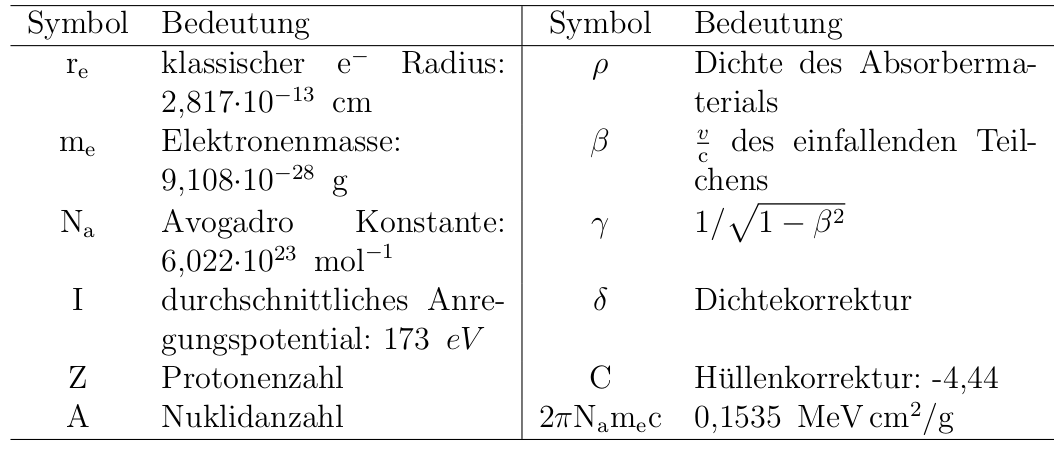
\includegraphics[width=\textwidth]{content/graphics/Bloch.png}
  \caption{Erklärung und Bedeutung der in Formel \eqref{eqn:bloch} verwendeten
  Parameter zur Bestimmung des Energieverlusts pro Wegstecke von Elektronen
  bei Durchgang durch ein Medium \cite{Anleitung}.}
  \label{fig:TabelleBloch}
\end{figure}

Der Parameter $\tau$ beschreibt die kinetische Energien und besitzt die Einheit $\text{m}_\text{e} c^2$.
Die Funktion $ \text{F}\left(\tau \right)$ ist ebenfalls genau bestimmt.
Die Bethe-Bloch-Gleichung ist eine materialspefizische Gleichung, die nicht nur
von der Energie des einfallenden Teilchens abhängt, sondern auch von den durch das
Material vorgegebenen Materialgegebenheiten. Bei der Berechnung eines
einfallenden Teilchens aus dem $^{90}\text{Sr}$ Primärzerfall, mit maximaler
Zerfallsenergie, ergibt sich eine durchschnittliche Energiedeposition pro
Wegstrecke in reinem Silizium von $\SI{3.88}{\mega\electronvolt\per\centi\meter}$.

\subsubsection{Energieverteilung in einem Silizium-Sensor}

Bei der Betrachtung der Energieverteilung eines Elektrons in einem
Siliziumsensors müssen einige mathematische Überlegungen gemacht werden. Der
zentrale Grenzwertsatz besagt, dass die Summe vieler identisch verteilter
Zufallsvariablen mit endlicher Varianz, näherungsweise einer Gaußverteilung
entspricht \cite{Grenzwert}. Übertragen auf das Problem, bedeutet das, dass eine
Normalverteilung für das Energiespektrum der deponierten Energie von den
geladenen Teilchen für eine ausreichende Dicke des Detektors zu erwarten ist.
Allerdings ist das hier nicht der Fall, da die Streifen selber sehr dünn sind
$\left(\SI{300}{\micro\meter}  \right)$ und es somit zu wenigen Stoßprozessen
kommt. Ein wichtiger Faktor dabei ist, dass die sekundär produzierten
Delta-Elektronen auf Grund der geringen Dicke des Sensors möglicherweise nicht
vollständig abgebremst werden und somit nicht die komplette Energie des Primärteilchens
deponiert wird. Es ergibt sich somit eine Energieverteilung, die asymmetrisch
verteilt ist, und ihren Peak näher an kleineren Energien finden und Ausläufer
zu hohen Energien aufweist, eine sogenannte Landauverteilung. \par \smallskip

Ebenfalls nicht zu vernachlässigen ist die statistische Energieverteilung der
Beta-Teilchen. Diese beeinflusst das Energiespektrum, wodurch eine Faltung
der Gaußverteilung mit der Landauverteilung die beste Beschreibung für das
Problem liefert.
Eine Charakteristik der Landauverteilung ist, dass der wahrscheinlichste Wert,
also der Ort des Peakes, näher an kleineren x-Werten (hier also Energien) liegt,
als der Mittelwert der Verteilung. Dieser Fakt stammt aus der Asymmetrie
der Verteilung. In diesem Versuch werden keine Energien direkt gemessen. Gemessen
wird zunächst in Einheiten der Ausgabe des Analog-zu-Digital-Konverters, sogenannten ADC.
Die ADC Counts können dann mit dem Wissen, dass die Energie zur Erstellung eines
Elektron-Loch-Paares in Silizium $\SI{3.6}{\electronvolt}$ beträgt, in
Energien umgerechnet werden.
\newpage
